% ------------------------------------------------------------------------------
% The OpenQuake Book
% 
%
% Document distributed under the Common Creative License bla bla bla
% ------------------------------------------------------------------------------
\documentclass[12pt,a4paper,smallheadings]{scrbook}
% --------------------------------------------------------------------- Packages
\usepackage{amsmath}
\usepackage{titlesec}
\usepackage{a4}
\usepackage[dvips]{graphicx}
% Solves problems with margin notes
\usepackage{mparhack} 
	\setlength{\marginparwidth}{1.1in}
	\let\oldmarginpar\marginpar
	\renewcommand\marginpar[1]{\-\oldmarginpar[\raggedright\color{red01}
	\footnotesize #1]%
	{\raggedright\footnotesize #1}}
% Colors
\usepackage{color}
	\definecolor{blue01}{rgb}{0,0,.5}
	\definecolor{gray01}{rgb}{0.1,0.1,0.1}
	\definecolor{red01}{rgb}{0.5,0.0,0.0}
\usepackage[italian,english]{babel}
%\usepackage[colorlinks=true]{hyperref}
%\usepackage{makeindex} % Used to create the index
%	\makeindex
\usepackage[square,colon]{natbib} % Used to 
\usepackage[labelfont=bf]{caption} % Used to reformat section typesetting
\usepackage{scrpage2}
	\lofoot[]{\includegraphics[width=2.0cm]{./Figures/openquake_logo1.eps}}
	\refoot[]{\includegraphics[width=2.0cm]{./Figures/openquake_logo1.eps}}
% - - - - - - - - - - - - - - - - - - - - - - - - - - - - - - - - Setting Fonts
\renewcommand{\encodingdefault}{OT1}
\renewcommand{\familydefault}{cmss}
\renewcommand{\seriesdefault}{m}
\renewcommand{\shapedefault}{up}
% - - - - - - - - - - - - - - - - - - - - - - - - - -  Reformatting PART Titles
\titleformat{\part}[display]
{\filleft\normalfont\sffamily}
{\textcolor{blue01}{\bfseries\large PART}\hspace{4pt}
	\bfseries\Huge\textcolor{blue01}{\thepart}}
{1pc}
{\Huge\bfseries\textcolor{blue01}}
[]
% - - - - - - - - - - - - - - - - - - - - - - - - - Reformatting CHAPTER Titles
% Titles: CHAPTER
\titleformat{\chapter}
	[display] % shape
	{\filleft\normalfont\sffamily} % format
	{\textcolor{blue01}{\bfseries\MakeUppercase{\chaptertitlename}} % label
		\hspace{4pt}\Huge\bfseries\textcolor{blue01}{\thechapter}} 
	{1pc} % sep
	{\Huge\bfseries\textcolor{blue01}} % Before
	[]
% - - - - - - - - - - - - - - - - - - - - - - - - - Reformatting SECTION Titles
% Titles: SECTION
\titleformat{\section}
	[hang] % shape
	{\vspace{.8ex}\Large\bfseries\color{blue01}} % format 
	{\textcolor{blue01}{\thesection.}} % label
	{.5em} % sep
	{} % before
	[] % after
% - - - - - - - - - - - - - - - - - - - - - - -  Reformatting SUBSECTION Titles
% Titles: SUBSECTION
\titleformat{\subsection}
	[hang] % shape
	{\vspace{.8ex}\large\bfseries\color{blue01}} % format 
	{\textcolor{blue01}{\thesubsection.}} % label
	{.5em} % sep
	{} % before
	[] % after
% - - - - - - - - - - - - - - - - - - - - - - - - - - - - - - - - - - - - - - - 
% Titles: SUBSUBSECTION
\titleformat{\subsubsection}
	[hang] % shape
	{\vspace{.8ex}\normalfont\bfseries\color{blue01}} % format 
	{} % label
	{.5em} % sep
	{} % before
	[] % after
% ------------------------------------------------------------------------------
\uppertitleback{
   \textbf{Authors:} \\
   Helen Crowley$^1$, Leonardo Garrido, Damiano Monelli, Marco Pagani$^1$, 
	Vitor Silva$^1$ \\ \hfill \\
   \small
   $^1$ GEM Foundation\\
   via Ferrata, 1 \\ 
   20133 Pavia \\
   Italy \\
   ($<$name.surname$>$@globalquakemodel.org)
   \normalsize
}  
%
% =============================================================== BEGIN DOCUMENT
% -------------------------------------------------- Title and table of contents
\begin{document}
\begin{titlepage}
	\titlehead{\emph{``OpenQuake: Shaken not stirred''}}
	\title{ \textcolor{blue01}{\textsf{\bfseries\Huge The OpenQuake Book}}  }
\end{titlepage}

\pagestyle{scrheadings}
\maketitle
\tableofcontents
%
% --------------------------------------------------------- Symbols and acronyms
\chapter*{Symbols and acronyms}
	\begin{tabular}{p{9.5cm}rr}
\bf{Quantity or Description} & \bf{Symbol or} & \bf{Unit of} \\ 
              & \bf{acronym}   & \bf{measure}  \\
Distance \dotfill & $D$ or $d$ & \text{km} \\ 
Frequency-Magnitude Distribution \dotfill & FMD & \\
Gutenberg-Richter (magnitude-frequency relationship) \dotfill & G-R &  \\
Ground motion (GM) or intensity measure type (IMT) \dotfill & $U$ or $u$ & g \\
Ground Motion Field \dotfill & GMF & \\
Ground Motion Prediction Equation \dotfill & GMPE &  \\
Magnitude \dotfill & $M$ or $m$ & \\
Natural hazards' Risk Markup Language \dotfill & nrML & \\
Occurrence Rate \dotfill & $\lambda$ & events/yr \\
OpenQuake \dotfill & OQ & \\
Rupture \dotfill & $rup$ & \\
Stochastic Event Set \dotfill & SES & \\
\end{tabular}

% ==============================================================================
% ------------------------------------------------------------------------- Part
\part{Introduction}
% ------------------------------------------------------------------------------
\chapter{OpenQuake background}
	% ------------------------------------------------------------------------------
An OpenQuake schema evidencing main inputs and calculators is represented in 
Figure \ref{fig:openquake_schema}.
% . . . . . . . . . . . . . . . . . . . . . . . . . . . . . . . . . . . > Figure
\begin{figure}
\includegraphics[width=17cm,angle=90]{./Figures/engine8_20101123.eps}
\caption{OpenQuake schema. Purple boxes are the calculators included in the  
the hazard part of OQ; green boxes are the risk calculators. The method of 
\citet{wesson2009} is represented in a separete box since it incorporates 
hazard and risk calculations.}
\label{fig:openquake_schema}
\end{figure}
% . . . . . . . . . . . . . . . . . . . . . . . . . . . . . . . . . . . < Figure

% ------------------------------------------------------------------------------
\chapter{Brief desciption of OpenQuake IT aspects}
	\input{./Part_Introduction/it.tex}
% ==============================================================================
% ------------------------------------------------------------------------- Part
\part{Hazard}
% ------------------------------------------------------------------------------
\chapter{Introduction}
	%
Introduction to the hazard component of OpenQuake

% ------------------------------------------------------------------------------
\chapter{OpenQuake input description}
	A PSHA input model contains four distinct information blocks: (1) information 
regarding location, geometry, and seismicity generation properties of seismic
sources, (2) information about ground motion prediction equations to be 
adopted in the calculation, (3) information about the epistemic uncertainties 
related to the two aforementioned points, and (4) information specifying 
calculation settings.

The description of OpenQuake seismic source properties is subdivided into 
source location and geometry and source frequency-magnitude distribution. 
Section \ref{hazard:seismic_source_types} provides an in deep description of 
the properties pertinent to the different source types supported together 
with examples of each single source type nrML description. 

The selection of ground motion prediction equations (GMPE) to be used in an 
hazard analysis in OpenQuake is basically accomplished using a label.  
The user can associate a GMPE to each tectonic region considered in the 
analysis (Active Shallow tectonic, Stable Continental etc.). Examples of 
GMPEs selection are provided in section \ref{hazard:gmpe_selection} at page 
\pageref{hazard:gmpe_selection}.

The description of epistemic uncertainties is accomplished via a logic-tree 
structure, described by branching level. Further explanations on the way we 
model logic-tree is provided in section \ref{hazard:logic_tree} at page 
\pageref{hazard:logic_tree}. 

The last, but not less important, block of information characterizing a PSHA 
input model contains parameters specifying the way calculations must be 
carried out. The information to be included in this part of the input is 
strictly related to the calculation properties of the engine. Section 
\ref{hazard:calculation_settings} provides an outlook of the hazard specific 
calculation setting supported by OpenQuake. 
%
% ------------------------------------------------------------------------------
\section{Seismic source typologies description}
\label{hazard:seismic_source_types}
OpenQuake at present time provides four seismic source typologies, for the 
most part defined in the course of the GEM1 project \citep{pagani2010}:
\begin{itemize}
\item Area source - This source type is the one that - at least for the time 
being - is most frequently adopted in national and regional PSHA models.
\item Grid source - Grid sources can be considered a replacement for area 
sources since they both model distributed seismicity;
\item Simple fault sources - Simple faults are the easiest modality available
to specify the parameters need to characterize a fault source. This typology
is usually adopted to describe shallow seismogenic fault sources.
\item Complex fault sources - Complex faults is usually adopted to model
subduction interface sources with a complex geometry. 
\end{itemize}

The basic assumptions adopted in the definition of these source typologies 
are the following:
\begin{itemize}
\item In the case of area and fault sources, the seismicity is homogeneously 
distributed over the source; 
\item Seismicity temporal occurrence follows a Poissonian model; 
\item The frequency-magnitude distribution can be approximated to a evenly 
discretized distribution. 
\end{itemize}
%
%  - - - - - - - - - - - - - - - - - - - - - - - - - - - - - - - - - - - - - - - 
\subsection{Area sources}
\label{hazard:seismic_source_types:areaSources}
Area sources usually model the seismicity occurring over wide areas where fault 
sources identification or characterization - i.e. the unambiguous definition 
of seismicity occurrence parameters - is difficult. 

The \citet{sshac1997} defined three main types of area seismic sources using as 
a discriminant their extension:
\begin{enumerate}
\item Area sources enclosing concentrated zones of seismicity;
\item Regional area sources;
\item Background area sources.
\end{enumerate}
As a general rule, the criteria - and the related uncertainties - adopted for 
their definition varies according to each area source type. From a hazard 
computation standpoint we do not introduce any difference between these three 
area types.
	\marginpar{marco: In the future we may support a specialized background 
	area source type}
%
%  . . . . . . . . . . . . . . . . . . . . . . . . . . . . . . . . . . . . . . . 
\subsubsection{Parameters}
\begin{itemize}
\item A polygon that identifies the external border of the area. Eventually, 
internal borders can be specified so as to create holes inside an area.
	\marginpar{marco: I don't think nrML supports area sources with holes.}
\item One (or many) couples of the following objects:
\begin{itemize}
	\item A discrete Frequency-Magnitude Distribution (FMD)
	\item Strike, dip, and rake angles characterizing the seismicity specified 
	in the associated FMD and occurring in the area source under consideration. 
	For example, \cite{coppersmith2009} defines a discrete 
	distribution of strike values (dip is not considered because the source-site 
	metrics they use is the Joyner-Boore distance). 
\end{itemize}
This area source specification permits the accurate characterization of 
seismicity occurrence within an area by explicitly distributing the seismicity 
on the existing faulting trends. 
\item An array to specify the depth to the top of rupture dependency on magnitude. 
The array contains two columns and one or many $<$depth, magnitude$>$ tuples. 
Each tuple specifies the depth to the top of rupture for magnitudes equal or 
greater than the specific value. 
\item A value to indicate the hypocentral depth in case of punctual sources. 
By convention all the events with magnitude lower than the lowest value contained 
in the array used to specify the depth to the top of rupture are modelled 
considering a punctual source. On the opposite, ruptures with magnitude equal or 
greater than the lowest value of magnitude contained in the depth to the top of 
rupture array are modelled considering their finite dimensions. 
\end{itemize}
%
%  - - - - - - - - - - - - - - - - - - - - - - - - - - - - - - - - - - - - - - - -
\subsection{Grid sources}
A grid source is a typology used to model distributed seismicity - usually 
of low and intermediate magnitude.

Grid sources can be considered as a PSHA source model alternative to area 
sources since they both try to represent distributed seismicity. Grid sources 
usually derive from the application of seismicity smoothing algorithms 
\citep{frankel1995,woo1996}. 

The use of these algorithms carries some advantages compared to area sources, 
indeed, (1) they remove most of the unavoidable degree of subjectivity due to 
the definition of the geometries and (2) they define a seismicity spatial 
pattern that is, usually, more similar to reality. Nevertheless, some smoothing 
algorithms require the a-priori definition of some setup parameters that expose 
the calculation to a certain partiality level.

Grid source models are modelled in OpenQuake simply as set of 
point sources. The next section describes the parameters required to 
characterize a point source.
%
%  . . . . . . . . . . . . . . . . . . . . . . . . . . . . . . . . . . . . . . . 
\subsubsection{Parameters}
For each grid node:
\begin{itemize}
\item A location specified in terms of the <latitude,longitude> tuple;
\item Similarly to area sources, one (or many) couples of the following objects:
	\begin{itemize}
	\item A discrete Frequency-Magnitude Distribution (FMD)
	\item Strike, dip, and rake angles characterizing the seismicity specified 
	in the associated FMD. 
	\end{itemize}
\item An array to specify the dependency on magnitude of the depth to the top of 
	rupture. This array contains two columns and one or many 
	$<$depth, magnitude$>$ tuples where each tuple specifies the depth to the 
	top of rupture for magnitudes equal or greater than a specific value. 
\item A value to indicate the hypocentral depth in case of punctual sources. The 
	same convention specified for area sources applies here. 
\end{itemize}
%  - - - - - - - - - - - - - - - - - - - - - - - - - - - - - - - - - - - - - - - -
\subsection{Accounting for rupture finiteness in case of areal and grid sources}
In the scientific literature is well known that for magnitudes approximately 
greater than six the finite dimension of the rupture cannot be neglected in 
the calculation of the source-site distance. 
	\marginpar{marco: it's not clear if and how much ruptures can extend
	outside the area border}

To correctly calculate the source-site distance in case of area and grid sources 
two are the approaches available. The first is to multiply the epicentral or 
hypocentral distance by a correction factor (see for example \cite{harmsen08})
the second requires to place on each node a number of ruptures with different 
orientation. 



%  - - - - - - - - - - - - - - - - - - - - - - - - - - - - - - - - - - - - - - - -
\subsection{Simple faults}
Faults 
%
%  . . . . . . . . . . . . . . . . . . . . . . . . . . . . . . . . . . . . . . . 
\subsubsection{Parameters}
\begin{itemize}
\item A fault trace (usually a multi-segment line) 
\item A FMD 
\item An average value of the dip angle  (Aki-Richards convention; see 
	\citet{aki2002}),
\item Rake angle (Aki-Richards convention; see \citet{aki2002}) 
\item Upper and lower values of depth limiting the seismogenic interval 
\item A boolean flag that specifies if ruptures should follow a magnitude scaling 
relationship and thus be distributed homogeneously over the fault surface or it is 
accepted that ruptures of whatever magnitude (of course of the ones admitted by 
the FMD) will rupture the whole fault surface.
\end{itemize}
%  - - - - - - - - - - - - - - - - - - - - - - - - - - - - - - - - - - - - - - - -
\subsection{Complex faults}
Complex faults differ from simple fault just by the way geometry is described and, 
consequently in the way the fault surface is created. The input parameters used to 
describe complex faults are, for the most part, the same used to describe the 
simple fault typology. In particular, in the case of complex faults the dip angle
is not requested while the fault trace is substituted by two fault traces used to 
limit at top and bottom the fault surface. 
%  - - - - - - - - - - - - - - - - - - - - - - - - - - - - - - - - - - - - - - - -
\subsubsection{Representation of complex faults}
Usually, we use complex faults to model intraplate megathrust faults such as the 
big subduction structures active in the Pacific (Sumatra, South America, Japan).
%
% ------------------------------------------------------------------------------
\section{GMPEs description}
\label{hazard:gmpe_selection}
%
% ------------------------------------------------------------------------------
\section{Logic-tree description}
\label{hazard:logic_tree}
%
% ------------------------------------------------------------------------------
\section{Calculation settings description}
\label{hazard:calculation_settings}


% ------------------------------------------------------------------------------
\chapter{Earthquake Rupture Forecast calculator}
	\index{Source Model}
\index{Source Model!Inital (ISM)}
%
The calculation of the Seismicity Occurrence Model (i.e. ERF) starts from a Source model. 
%
The creation of a Source Model in OpenQuake is done by a calculator, named Logic Tree Processor (LTP). The LTP uses one of the ISMs and the logic tree structure included in the Source System to create Source Model.
%
A Source Model is a complete description of the type, geometry and seismicity occurrence properties of the seismic sources necessary to calculate comprehensively the hazard over the investigated area. In a Source Model is not possible to inc epistemic uncertainties.

Once a Source Model is created, using the Earthquake Rupture Forecast calculator we create a list of the ruptures that can be generated by all the sources included in the Source Model. Each rupture is associated with a probability of occurrence in the time span specified in the calculation settings. 
 

The Earthquake Rupture Forecast calculator creates  computes for each rupture the probability of occurence in a time span specified in the configuration file.
The list of ruptures correponds to all the possible ruptures that can be generated by the all the seismic sources included in Source Model can generate.
%
Each rupture has 


%
% ------------------------------------------------------------------------------
\section{The Logic Tree processor}
Logic Tree processor

%
% ------------------------------------------------------------------------------
\section{ERF calculator}

%
%  - - - - - - - - - - - - - - - - - - - - - - - - - - - - - - - - - - - - - - -
\subsection{ERF creation in case of Grid sources}
Area sources (see also Section \ref{hazard:seismic_source_types:areaSources} 
at page \pageref{hazard:seismic_source_types:areaSources}) 

%
%  - - - - - - - - - - - - - - - - - - - - - - - - - - - - - - - - - - - - - - -
\subsection{ERF creation in case of Grid sources}

%
%  - - - - - - - - - - - - - - - - - - - - - - - - - - - - - - - - - - - - - - -
\subsection{ERF creation in case of Fault sources}

%
%  . . . . . . . . . . . . . . . . . . . . . . . . . . . . . . . . . . . . . . .
\subsubsection{Fault sources with simple geometry}

%
%  . . . . . . . . . . . . . . . . . . . . . . . . . . . . . . . . . . . . . . .
\subsubsection{Fault sources with complex geometry}

% ------------------------------------------------------------------------------
\chapter{Classical PSHA calculator}
	OpenQuake computes hazard based on the classical PSHA approach 
\citep{cornell1968,mcguire2004} following the methodology proposed by 
\citet{field2003}. This methodology has the distinctive property of performing
the entire calculation using probabilities, as orginally proposed by 
\citet{chiang1984}, instead of working with occurrence rates like in common
PSHA codes \citep[see for instance][]{bender1987}. 
This has the clear advantage of decoupling the creation of the probabilistic 
seismicity occurrence model (in the OpenSHA terminology this is defined as the 
Earthquake Rupture Forecast) from the assumption of a Poissonian temporal 
occurrence model. \citet{field2003} demonstrated the congruence between the 
original PSHA formulation based on occurrences and the methodology here adopted 
in the case of a Poissonian temporal model. 

From a more strict calculation perspective two, are the main steps accomplished:
\begin{itemize}
\item Creation of the probabilistic seismicity occurrence model, i.e. a discrete 
distribution giving the probability of occurrence of each possible rupture 
occurring on one of the seismic sources defined in the PSHA input model in a  
given time span.  
\item Calculation of hazard at the site by combining the probabilistic 
occurrence model with a ground motion prediction equation (also Intensity 
Measure Relationship in the OpenSHA jargon).
\end{itemize}
%
% --------------------------------------------------------------------------------
\section{Calculation kernel}
Considering a single rupture $rup$ sof magnitude $m_i$ occurring on a given seismic 
source, it's probability of occurrence in a given time span is: 
\begin{equation}
P(Rup) = P(n=1)\,P(M=m_i)\,P(Rup|m_i)
\end{equation}
where $P(n=1)$ is the probability of occurrence of one event in the given seismic
source, $P(M=m_i)$ is the probability that given an occurrence this will have a 
magnitude equal to $m_i$ and, $P(Rup|m_i)$ is the probability of rupture $Rup$
given magnitude $m_i$ within the seismic source considered 
%
% --------------------------------------------------------------------------------
\section{Hazard calculation: traditional formulation in terms of probabilities}
Following \cite{field2003}, the traditional formulation in terms of probabilities:
%
\begin{equation}
P(U\geq u)= 
	1-\prod\limits_{i=1}^{l} 
	\left[\sum\limits_{s=0}^{+\infty}
	\left(P(S=s) 
	\left(
		1-\sum\limits_{j=0}^{j(i)}\sum\limits_{s=0}^{K(i,j)} 
		P(m_{i,j}) 
		P(R_{i,j,k}|m_{i,j}) P(U\geq u|m_{i,j},R_{i,j,k})
	\right)
	\right)^{s}
	\right] 
\end{equation}
where $l$ i the number of sources 

If the probability of multiple occurrences is assumed to be negligible:
%
\begin{equation}
P(X\geq x)=1-\prod\limits_{i=1}^{l} 
	\left( 
		1-\sum\limits_{n=1}^{N(i)}P(Rup_{i,n})P(X\geq x|Rup_{i,n})
	\right)
\end{equation}

%  - - - - - - - - - - - - - - - - - - - - - - - - - - - - - - - - - - - - - - - -
\subsection{Example}
In case of two punctual sources each one generating a single rupture, the 
probability of exceedance of ground motion $u$ in a given site corresponds to:
%
\begin{eqnarray}
P(U\geq u)=
	1-
	\biggl(& 
		\bigl[ 1-P(Rup_{i,1})P(U\geq u|Rup_{i,1}) \bigr] \nonumber \\
		& \bigl[ 1-P(Rup_{i,2})P(U\geq u|Rup_{i,2}) \bigr]
	\,\biggr)
\end{eqnarray}
% ------------------------------------------------------------------------------
\chapter{Stochastic event set and ground motion field calculators}
	The calculation of stochastic event sets and the corresponding ground motion fields is a methodology tightly connected with a specific seismic risk analysis of common use within the insurance and re-insurance industry (CITATION). 
%
OpenQuake given an Earthquake Rupture Forecast can generate a number of seismicity histories, each one representing a possible realisation of the seismicity that the sources included in a Source Model can generate within a given time span (fixed by the user).
% 
The 

Each rupture in a seismicity history is successively associated with a ground motion field, an object describing the spatial distribution of a scalar parameter representative of the intensity of shaking (e.g. PGA or Spectral Acceleration). OpenQuake has the capability to generate 
%
% ------------------------------------------------------------------------------
\section{Stochastic Event Set Calculator}
The Inverse Trasform CITATION is a methodology widely used to randomly sample 
a discrete probabilistic distribution 

%
% ------------------------------------------------------------------------------
\section{Ground Motion Fields calculator} 
We generate ground motion fields using the 
%
%  - - - - - - - - - - - - - - - - - - - - - - - - - - - - - - - - - - - - - - -
\subsection{Spatially correlated ground motion fields}
The genearation of spatially correlated ground motion fields is based on the work of \citet{jayaram2009} where they propose a model - based on a semivarigram - for describing 
\begin{equation}
\gamma(h) = a \left[1-\exp\left(-\frac{3h}{b}\right)\right]
\end{equation}

%
% ------------------------------------------------------------------------------
\section{Stochastic PSHA calculator} 
The OpeQuake stochastic PSHA calculator provides a way to check the consistency between the result provided by a classical PSHA calculator and the results that can be obtained by a number of ground motion fields, representative of the 

% ------------------------------------------------------------------------------
\chapter{Wesson et al. [2009] risk calculation implementation}
	%
In the procedure proposed by \cite{wesson2009} the creation of the ERF follows the 
classical approach.

Using an ERF, for each rupture $Rup$ is possible to calculate the 
probability that a given ground motion $U$ is in the interval $u_x\pm \Delta u$ 
given an inter-event variability $\epsilon_{inter}$ (this corresponds to 
equation 3 of \cite{wesson2009}): 
%
\begin{eqnarray}
P(u_x-\Delta u\leq U<u_x+\Delta u|Rup,\epsilon_{inter}) & = &  
	\Phi\bigg(\frac{(\ln (u_x-\Delta u)-\ln(u_0)}{\sigma_{intra}}\bigg) - \nonumber \\
	& - & \Phi\bigg(\frac{(\ln (u_x+\Delta u)-\ln(u_0)}{\sigma_{intra}}\bigg) 
\end{eqnarray}
where $\ln(u_0)$ is the mean of the GMPE computed considering a value 
$\epsilon_{intra}$ and a rupture $Rup$, (generally characterized by a geometry 
and a magnitude) and $\Phi$ is the standard normal CDF. 
  
The next step is to calculate the PMF of losses for a given rupture. Given an asset, 
the probability of suffering a loss value in the interval $[l-\Delta l, l+\Delta[$ 
given a ground motion value in the interval $[u_x-\Delta u,u_x+\Delta u[$ (note that in this 
case the distribution of ground motion $u$ will depend on $\epsilon_{intra}$) 
corresponds to:
%
\begin{equation}
\begin{array}{rl}
P(l-\Delta l\leq L < & l-\Delta l|Rup,\epsilon_{inter}) = \\
 	\sum\limits_{x=0}^{\infty}  
	& P(l-\Delta l\leq L < l-\Delta l|u_x+\Delta u\leq U<u_x+\Delta u) \\
	& P(u_x-\Delta u\leq U<u_x+\Delta u|R,\epsilon_{inter})) \\
\end{array}
\end{equation}
%
If $P^i(L=l|Rup,\epsilon_{inter})$ corresponds to the conditional probability mass
function describing the discrete probability of having a loss in the interval 
$[l-\Delta l, l-\Delta[$ for the asset with index $i$, the probability of cumulated 
losses to a portfolio can be computed as:
\begin{equation}
P_{CL}(CL=cl|M,\epsilon_{inter})=P^1(L=l|Rup,\epsilon_{inter})*\ldots*P^n(L=l|Rup,
	\epsilon_{inter})
\end{equation}
where symbol $*$ stands for convolution. 

Finally, the total probability of exceeding a given level of cumulated losses $cl$ 
computed considering the contributions of all the ruptures occurring on all the 
seismic sources considered is (note that this expression extends equation A10 of
\cite{field2003}):  
%
\begin{equation}
P(CL\geq cl)=1-\prod\limits_{i=1}^{n} 
	\left( 
		1-\sum\limits_{n=1}^{N(i)}
		\sum\limits_{k=-3}^{3}
			P(Rup_{i,n})P(CL\geq cl|Rup_{i,n},\epsilon_k)
	\right)
\end{equation}
where $P(CL\geq cl|Rup_{i,n},\epsilon_k)$ can be simply derived from the PMF 
$P_{CL}(CL=cl|M,\epsilon_{inter})$, $n$ is the number of seismic sources.

% ==============================================================================
% ------------------------------------------------------------------------- Part
\part{Risk}
\chapter{Deterministic event based calculator}
	The deterministic event-based calculator is capable of computing losses and loss statistics for a single event for a collection of assets. Depending of the type of hazard input that is provided, two separate approaches can be followed. In the first one, the calculator uses two maps, one with the distribution of the mean ground motion and a second one with the associated aleatory variability. In the second approach, the event is repeated many times to model the variation in the inter-event variability and for each event, a ground motion field is generated taking into account the intra-event variability (and possibly the spatial correlation of the latter). The following scheme presents the architecture of this calculator:

\begin{figure}[ht]
\centering
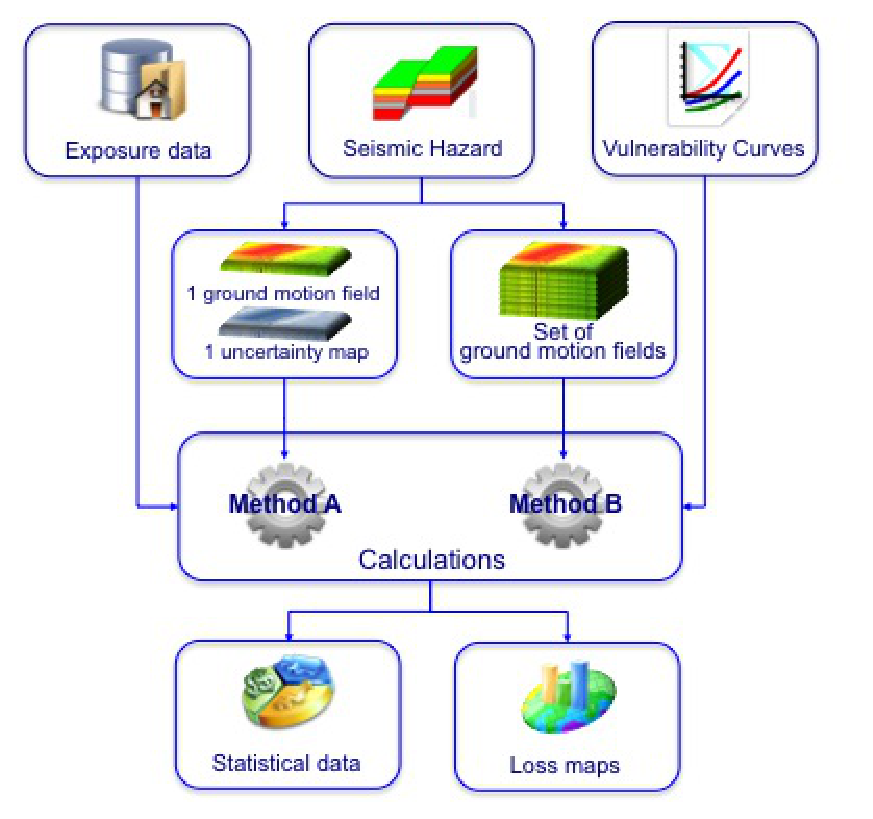
\includegraphics[width=9cm,height=9cm]{./Figures/Part_Risk/Scheme_Deter_calc.eps}
\caption{Architecture of the deterministic event-based calculator.}
\label{fig:Scheme_deter_calc}
\end{figure}

\section{Method A} 
\subsection{Description}
In this approach, after providing the two aforementioned maps, the mean ground motion and coefficient of variation at each site are used together with the assigned vulnerability function for each asset  to calculate a mean loss ratio. The aleatory variability in the ground motion is combined with the uncertainty in the vulnerability functions through the total probability theorem in order to calculate the standard deviation of the loss ratio for each asset.

\subsection{Calculation workflow}

To compute the mean loss:

\begin{enumerate}
\item In order to compute the probability of occurrence of each intensity measure level defined on the vulnerability function, an upper and lower bound needs to be calculated for each value. The limits for an $IML_n$ can be given by the following formulae:

\begin{equation}
Lower bound = \frac{IML_n+IML_{n-1}}{2}
\end{equation}

\begin{equation}
Upper bound = \frac{IML_{n+1}+IML_{n}}{2}
\end{equation}

The following figure illustrates the intervals that were computed based on 4 intensity measure levels that comprise a given vulnerability function:

\begin{figure}[ht]
\centering
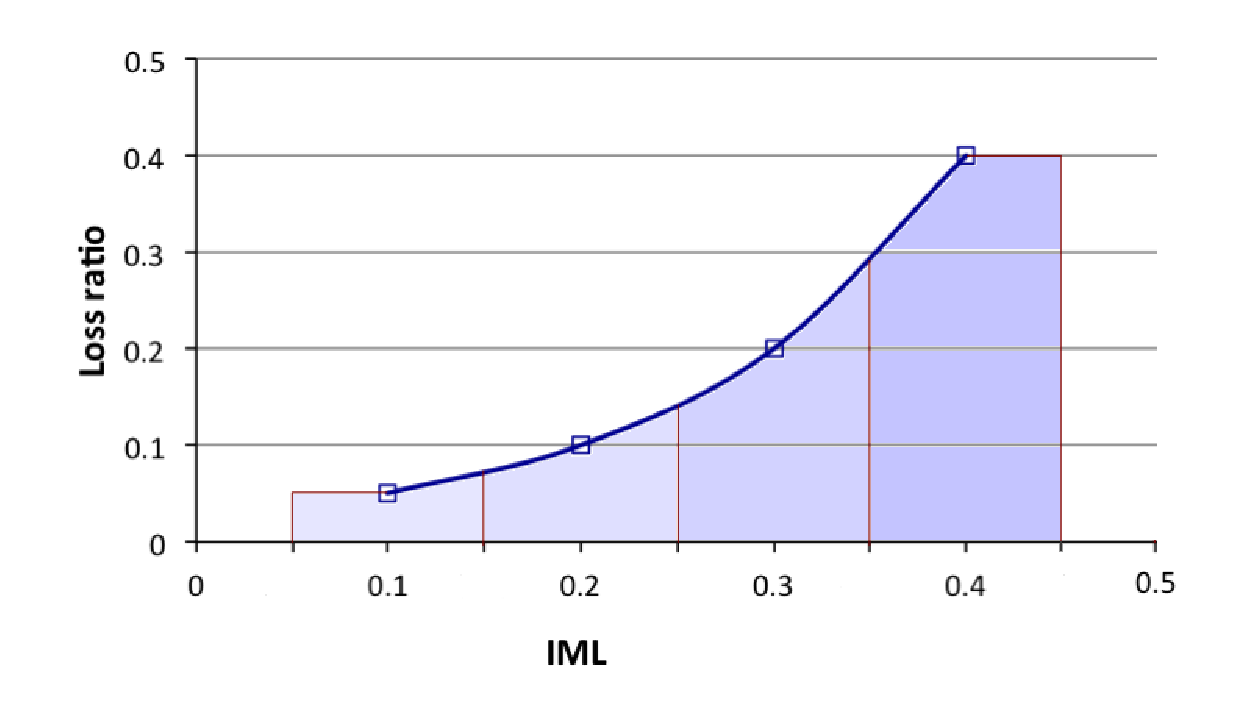
\includegraphics[width=8cm,height=5.5cm]{./Figures/Part_Risk/VF_intervals.eps}
\caption{Intervals for each intensity measure level on a discrete vulnerability function.}
\label{fig:VF_intervals}
\end{figure}

Note that for the first and last intensity measure level, there are no values before or after respectively. In this case, the lower and upper bound need to be computed based on the distance between the respective intensity measure level and the bound that was computed through one of the aforementioned formulae. Thus, the lower bound for the first intensity measure level can be given by:

\begin{equation}
Lower bound= IML_1-\frac{IML_2+IML_{1}}{2}
\end{equation}

And the upper bound for the last intensity measure level can be computed using:

\begin{equation}
Upper bound[IML_{n}]  = IML_{n}+\frac{IML_{n}-IML_{n-1}}{2}
\end{equation}

\item Once the intervals for each intensity measure level are defined, the probability of occurrence can be computed through the expression:

\begin{equation}
PO[IML_{n}]  = F(UB,\mu,\sigma)-F(LB,\mu,\sigma)
\end{equation}

Where $F$ stands for the cumulative distribution function, $UB$ and $LB$ stand for the upper and lower bound respectively of the $IML_n$ and $\mu$ and $\sigma$ stand for the logarithmic mean and standard deviation i.e. the mean ground motion and associated standard deviation of the normal distribution of the natural logarithm of the ground motion values.

\item Then, the mean loss ratio for each asset can be computed through the formula:

\begin{equation}
LR  = \sum_{n=1}^mPO[IML_n] \times LR_n
\end{equation}

\item The absolute mean loss can be computed by multiplying the mean loss ratio by the value of the asset contained on the exposure model file.

\end{enumerate}

To compute the standard deviation of the loss:

\begin{enumerate}
\item In order to compute this parameter, the total probability theorem needs to be used. The first step is to compute $E[LR_n^2]$, which is given by the following formula:

\begin{equation}
E[LR_n^2]=SD[LR_n]^2+E[LR_n]^2
\end{equation}

Where $SD[LR_n]$ stands for the standard deviation of the distribution of loss ratios and $E[LR_n]$ stands for the mean loss ratio.

\item Then, the total $E[LR^2]$ can be derived using the formula:

\begin{equation}
E[LR^2]=\sum_{n=1}^mPO[IML_n] \times E[LR_n]^2
\end{equation}

\item Subsequently the standard deviation of the loss ratio can be computed using the expression:

\begin{equation}
SD[LR]=\sqrt{E[LR^2]-E[LR]^2}
\end{equation}

Where $E[LR]$ stands for the mean loss ratio computed previously.

\item The absolute standard deviation of the loss can finally be computed by multiplying the standard deviation of the loss ratio by the value of the respective asset.

\end{enumerate}

\section{Method B}
\subsection{Description}
In this approach, for each ground motion field, the intensity measure level at a given site is used to calculate the mean and standard deviation of loss ratio using the vulnerability functions for each asset contained in the exposure file. Using these results, the mean and standard deviation of loss ratio across all events can be calculated. Again, loss ratios are converted into losses by multiplying by the value of the asset given in the exposure file. For this method, it is possible to aggregate the losses throughout the region and to compute the standard deviation of the aggregated loss. 

\subsection{Calculation workflow}

To compute the mean loss:

\begin{enumerate}
\item For each ground motion field, the intensity measure levels are related with the vulnerability functions to compute the mean loss ratio for each asset. Since currently the vulnerability functions are being defined in a discrete way, it is quite probable that the intensity measure level provided by the ground motion field is not contained in the vulnerability function. In these cases, linear interpolation methods are being employed to derive the mean loss ratio at the intensity measure level of interest.

\item The mean loss ratio for each asset across all possible simulations of the deterministic event can be calculated through the formula:

\begin{equation}
LR=\frac{\sum^m_{n=1}LR_n|IML}{m}
\end{equation}

Where $m$ stands for the number of ground motion fields simulated.

\item The mean loss can then be derived by multiplying the mean loss ratio by the value of the asset contained in the exposure model file.

\end{enumerate}

To compute the standard deviation of the loss:

\begin{enumerate}

\item Again, the total probability theorem is employed. $E[LR_n^2]$ is computed using the following formula:

\begin{equation}
E[LR_n^2]=SD[LR_n]^2+E[LR_n]^2
\end{equation}

Where $SD[LR_n]$ stands for the standard deviation of the distribution of loss ratios and $E[LR_n]$ stands for the mean loss ratio (for each ground motion field).

\item Then, the total $E[LR^2]$ can be derived using the formula:

\begin{equation}
E[LR^2]=\frac{\sum_{n=1}^m E[LR_n]^2}{m}
\end{equation}

\item The standard deviation of the loss ratio can be computed using the expression:

\begin{equation}
SD[LR]=\sqrt{E[LR^2]-E[LR]^2}
\end{equation}

Where $E[LR]$ stands for the mean loss ratio computed previously.

\item The standard deviation of the absolute loss can finally be computed by multiplying the standard deviation of the loss ratio by the value of the respective asset.

\end{enumerate}


% ------------------------------------------------------------------------------
\chapter{Probabilistic classical PSHA based calculator}
	\input{./Part_Risk/probabilistic_Classical_PSHA_Based.tex}
% ------------------------------------------------------------------------------
\chapter{Probabilistic event based calculator}
	\section{Description}
This method uses stochastic event sets and associated ground motion fields to compute loss curves for each asset contained in an exposure file, as illustrated in the following scheme:  

\begin{figure}[ht]
\centering
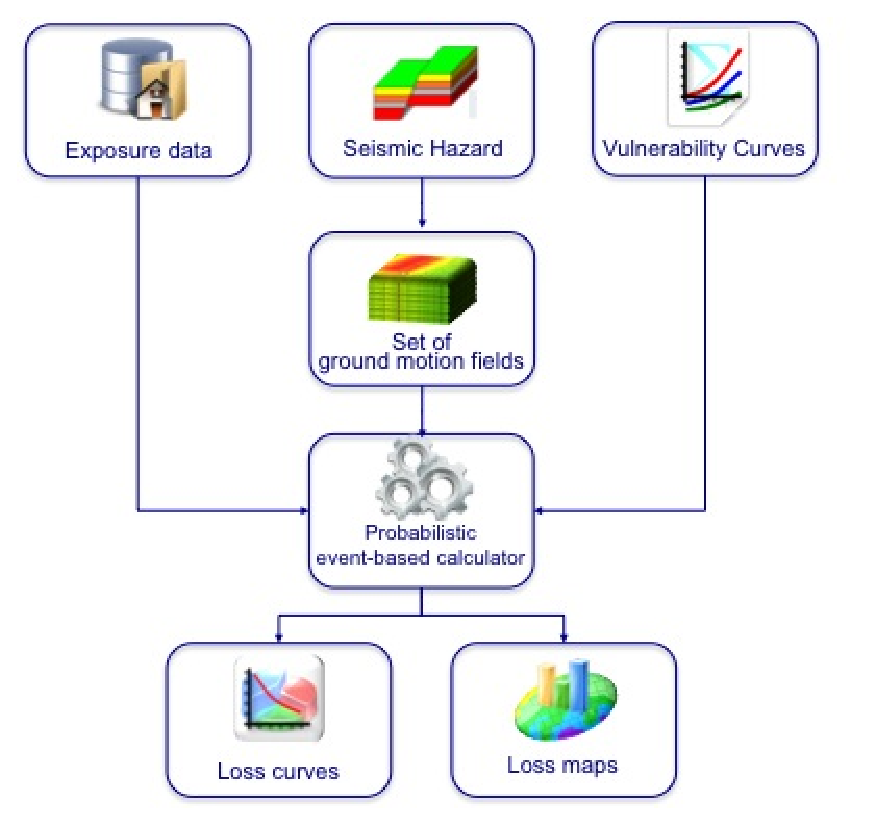
\includegraphics[width=9cm,height=10cm]{./Figures/Part_Risk/Scheme_Prob_calc.eps}
\caption{Architecture of the probabilistic event-based calculator.}
\label{fig:Scheme_Prob_calc}
\end{figure}

For each ground motion field, the intensity measure level at a given site is used to calculate the mean loss ratio using the vulnerability functions for each asset defined in the exposure file. The occurrence distribution of mean loss for a given asset is calculated using all of the ground motion fields, leading to a histogram of loss ratios which is then converted into a cumulative histogram, by calculating the number of cumulative occurrences for each interval of loss ratio. The rate of exceedance of each loss ratio is calculated by dividing the number of cumulative occurrences by the number of stochastic event sets multiplied by the length of each event set. By assuming a Poissionian distribution of the occurrence model, the probability of exceedance of each loss ratio is calculated. 
 
\par \ 

\par
 
If an aggregated loss curve for a portfolio of assets is required, a secondary module is required in order to aggregate the losses from all the assets in the exposure file, per event, before calculating the occurrence distribution of mean loss. If the assets are close enough, it is necessary to generate the ground motion fields taking into account the spatial correlation of ground motion residuals. 

\section{Calculations workflow}



% ==============================================================================
% ------------------------------------------------------------------------- Part
\part{Socio-Economic Impact Assessment}
	%
Introduction to the Socio-Economic Impact Assessment

% ==============================================================================
% ------------------------------------------------------------------------- Part
\part{Modeller's Toolkit}
% ------------------------------------------------------------------------------
\chapter{Introduction}
	%
Introduction to the hazard input Modellers' Toolkit

% ------------------------------------------------------------------------------
\chapter{Input visualization and preparation}
	%
% ------------------------------------------------------------------------------
\section{Hazard}
%
% ------------------------------------------------------------------------------
\section{Risk}
%
% ------------------------------------------------------------------------------
\section{Socio-Economic Impact}


% ==============================================================================
% ------------------------------------------------------------------------------
% ------------------------------------------------------------------------- Part
\part{Appendixes}
\appendix
\chapter{Example of OpenQuake hazard calculation configuration file}
	\input{./Part_Appendix/appendixHazardInputExample.tex}
% ------------------------------------------------------------------------------
\chapter{Example of OpenQuake risk calculation configuration file}
% ==============================================================================
% ----------------------------------------------------------------- Bibliography
\bibliographystyle{apalike}
\bibliography{/Users/marcop/seismology.bib}
\end{document}
